\chapter{Theoretical Background}

This chapter describes the fundamentals for the understanding of this paper. The cost estimation process in IT projects and the different methods to calculate the cost of a project are described in this chapter. The state of the art report combined with the market description will give a short overview over the situation about software estimation tools on the market and the possibility of a mobile solution of cost estimations. Android as the chosen platform and Java as the programming language will not be described in detail here and are assumed to be known.

\section{Cost estimation in software engineering}

The most expensive components of computer systems are software products. While private clients are mostly interested in the final price of a product, business clients of IT companies typically want to know the costs of the software before project launch. As analyzed in the \textit{IT-Trends} study from Capgemini \cite{capgemini} the IT budget of companies is growing up to 10\% every year. Whether developing a new project or standardizing existing software, the project costs are always on the main focus by the project management. As human resources is the biggest part of software costs, project managers and especially business clients want to know the estimated spendings and completion time of a project. Most of the estimation methods focus on this aspect and give the result in man days. These estimated days can then be converted into the real costs.
\\
Basically the cost estimation in software engineering wants to answer following questions:
\begin{enumerate}
\item How much effort is required to complete the project?
\item How much days are needed to complete the project?
\item What is the total cost of the project?
\end{enumerate}
While projects are a living thing, the effort may change due to unexpected difficulties. For a precise estimation of the total costs an adjustment cannot be avoided and it can be useful to change the estimation method in a later project phase. This means that the estimation process is not an one-time thing but will change through the life-time of a project. 


\subsection{Estimation Process}

It is common to create the first cost estimation before the system design, but also for monitoring purposes, milestones or if the client wants an overview of the project. Each time an actual cost estimation is needed the estimation process is executed which is a set of techniques and procedures that are used to derive the software cost estimate. Kathleen Peters described the basic process of an estimation, as seen in figure \ref{fig:basicEstimationProcess}, as it is common in the industry \cite{estimationProcess}.
As can bee seen from figure \ref{fig:basicEstimationProcess}, there are seven steps in the estimation process. The first part is to collect the initial requirements which is essential to know what the project is about and evaluate the approximate project size. With an selected estimation method, which are described in section \ref{chapter:estimationmethods}, the evaluated size of the project is then estimated. Afterwards the effort in man-days is calculated from which the cost schedule is created. Data from older projects can be included into the cost estimation. In the process step to approve the estimation, it has to be decided, if the costs are acceptable or if range of functions has to be shortened and the re-estimation has to bee started. If the cost estimation is acceptable the development of the product can start or continue.\\
\begin{figure}[h] 
	\centering 
	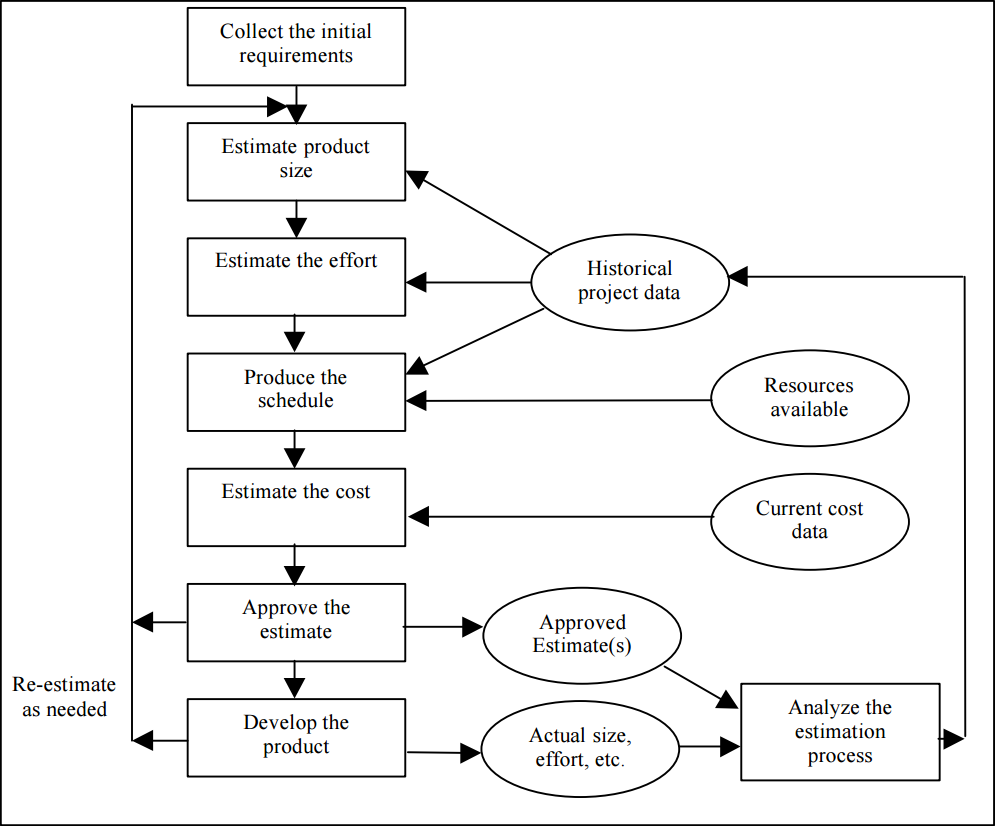
\includegraphics[width=13cm]{images/estimationProcess.PNG} 
	\caption{- The Basic Project Estimation Process}
	Source: Peters, Kathleen - Software Project Estimation, Page 3  
	\label{fig:basicEstimationProcess}
\end{figure}\\
In this classical view of the estimation process there are four outputs generated which can be described as following:
\begin{enumerate}
	\item Actual Size - the size of the project as a numerical value to make it comparable.
	\item Manpower Loading - the amount of personnel that is allocated to the project.
	\item Project Duration - the time that is needed to complete the project.
	\item Effort - the amount of effort required to complete the project is usually measured in units as man-days (MD) or person-months (PM).
\end{enumerate}
As described before, the estimation process can be triggered at any time in the project to re-estimate the costs. Depending on the project stage another estimation method than used before can be more precise.\\
The overview shown in fig. \ref{fig:estimationMethodInStage} shows that for example the SLIM method, is more suitable at the beginning of a project, whereas the ZKP method is more suitable after the system design stage. Most of the estimation methods can be used after the study stage. This is because a rough overview of the project size exists after the study stage. Different estimation methods may also change the evaluation output, which is one of the difficulties of cost estimations.\\
\begin{figure}[h] 
	\centering 
	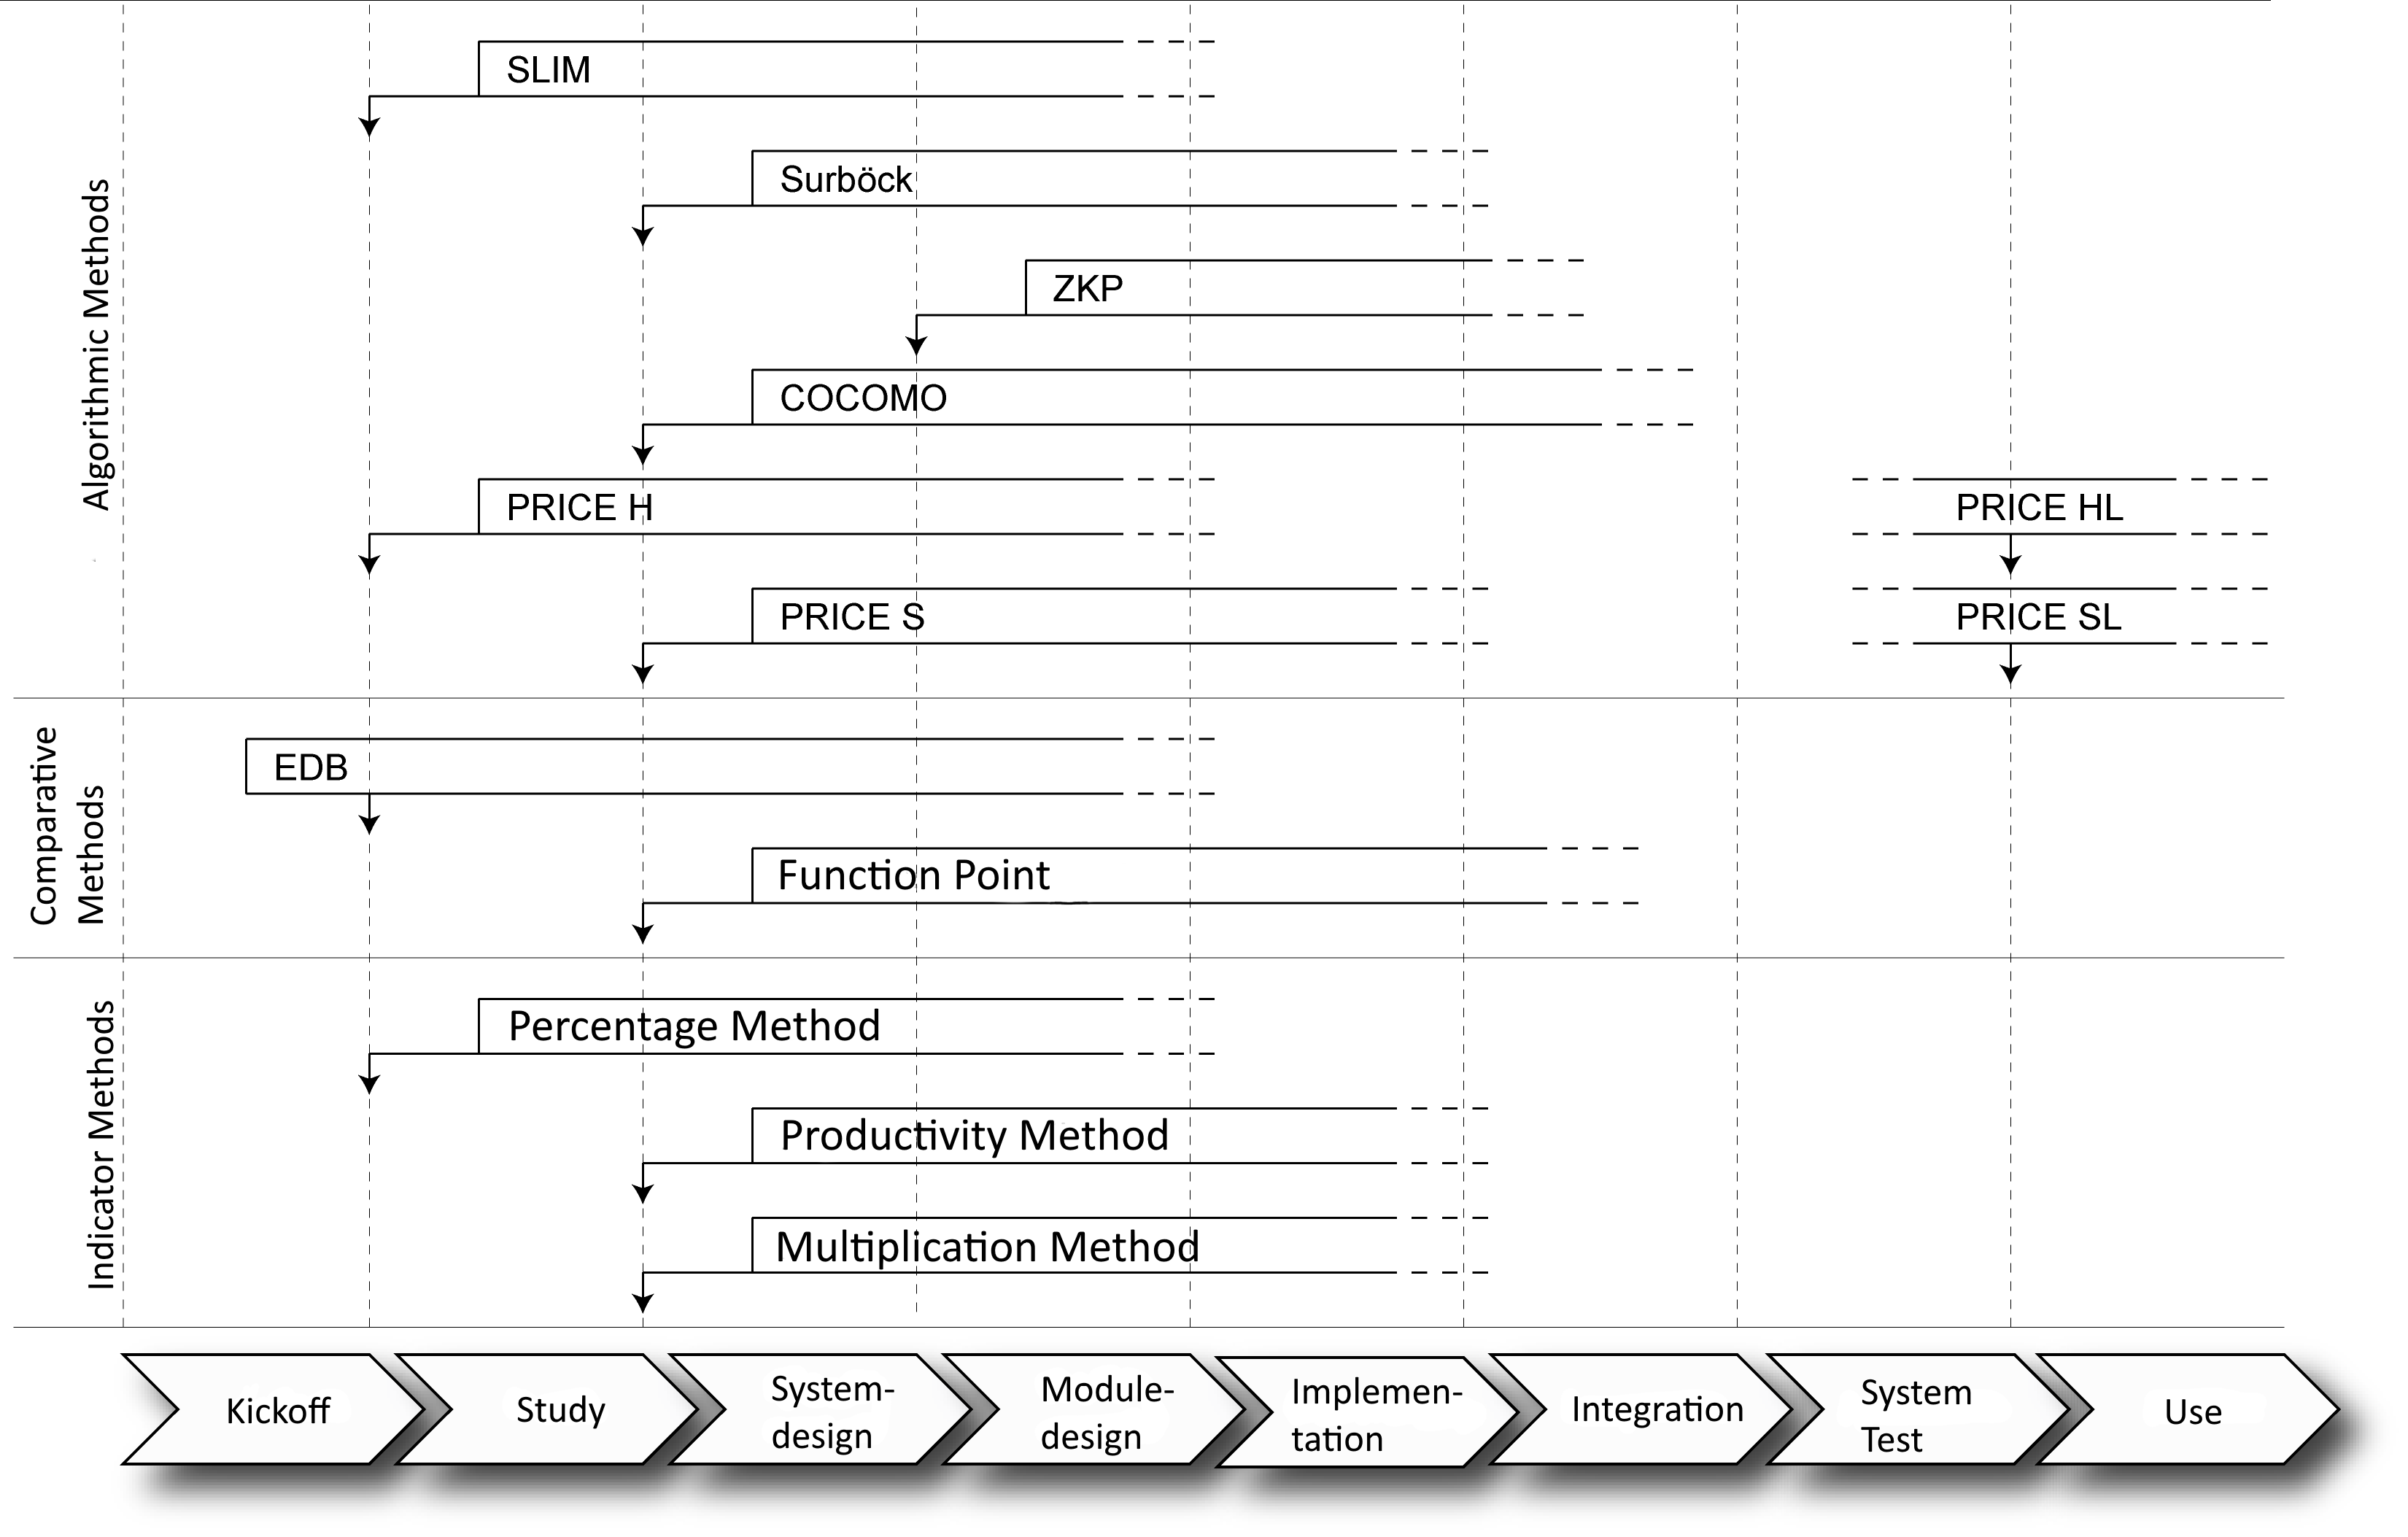
\includegraphics[width=13cm]{images/Einsatzzeitpunkte2.PNG} 
	\caption{- Starting Points of Estimation Methods} 
	Source: \url{http://winfwiki.wi-fom.de/index.php/Methoden_und_Verfahren_der_Aufwandsch\%C3\%A4tzung_im_Vergleich}
	\label{fig:estimationMethodInStage}
\end{figure}

\subsection{Difficulty of estimations}

One of the problems in estimating costs is that the actual code is only a small part of the project. Beside project planning there are many administrative tasks to do, like coordination of the project or searching and fixing errors. Most estimation methods evaluate the estimated time for the implementation only and too little or no time is evaluated for the non implementation tasks. This resolves in an underestimation of the non implementation tasks or an overestimation if they are predicted as a high value \cite{itplanung}.
\\
Most project managers rely on their experience from past projects. This is an advantage, but as technology changes fast and new projects inherit new problems there is no prior experience for some parts of the project. That can make experiences from prior projects useless. Because of the unique nature of projects it is common that a new project has big parts where no experience exists. Another difficulty of estimations is the fact that people who are inherited in the project have a more positive outlook and mostly underestimate the costs.
Also, customers often got a target time for the project, which leads in adjustment of the cost estimation. This leads to budget overrun if the needed resources are not available for the project \cite{winfwiki}.
\\
It is also not guaranteed that the estimated costs are accurate and stay within the budget. An estimation can easily go past their estimated target as new technologies and unexpected difficulties are commonplace. A partial requirements engineering can also cause an inaccurate cost estimation due to unexpected difficulties in the implementation.\\

\subsection{Methods for estimation}\label{chapter:estimationmethods}

Estimation methods are different metrics to calculate the costs of a project and there are different approaches to categorize the estimation methods. The categorization used in this paper is based on the book "Management von IT-Projekten" by Hans W. Wieczorrek, where the methods are subdivided in algorithmic, comparative, operating figures and expert discussion \cite{itplanung}.\\
All estimation techniques have in common, that only with a combined use of these different estimation methods a suitable result can be achieved as a measured value for the project. For the evaluation of the needed effort the underlying metric is used to calculate the effort for the project. On the basis of charge rates the effort size is calculated out of it.\\

\subsubsection{Algorithmic Method}

The algorithmic method uses a closed formula, which is based on empiric evaluation of already terminated projects or on existing mathematically models. Different forms of this method are the weight and the sampling method, which only differ in their usage.\\
The accuracy of the estimation depends primarily on the precision of the influence factors \cite{itplanung}. The algorithmic method always connects measurable project sizes, such as lines of code and implementable features, with influencing factors to get the result, represented as required effort in personnel costs. The basic formula, as described by Wieczorrek \cite{itplanung}:

\begin{equation}
	Personnel costs = f(result quantity, influencing factors)
\end{equation}

\subsubsection{Comparative Method}

Not based on a formula or numerical connection, the comparative method tries to create a reference between the current project and past projects. Therefore projects from the own company or the same industry sector are analyzed with appropriate comparison methods. This estimation method has the advantage, that it can be used early in project development \cite{itplanung}. This method can be used for hardware and software projects.

\subsubsection{Key Figures Method}

Estimation methods based on key figures can be differed to multiplier and percentage  method. The multiplier method uses units of power as the base to estimate the total expenditure, whereas the percentage method uses the effort of a project stage to estimate the effort for the next stage.\\
After project completion a post calculation determines the total project costs and the amount of specific types of costs. In order to calculate these costs, they will be divided by the scope of the developed product. This results in new key figures which can be used for new projects by multiplication of the estimated scope with the appropriate key figures. Regular actualization of the key figures is necessary for right results \cite{itplanung}.\\

\subsubsection{Expert Discussion Method}

As a quantitative and heuristic method the expert discussion uses knowledge from selected groups of people. It differentiates between four kinds: single person interview, multiple person interview, Delphi method and assessment meeting.\\
The advantage of this estimation method is, that they are useful for all project types. The problem with the expert discussion is, that this method is strongly affected by subjective opinions and the experience of the interviewees. As a result, expert discussions should never be used for complete projects but only for sub projects \cite{itplanung}.\\

\section{Estimation Techniques}

The existing estimation techniques rely on experience-based judgments by project managers
who created, by combining estimation methods, techniques can be used to estimate the effort of a project. Most of the estimation techniques became popular in the 80's, with the agile projects becoming more popular estimation techniques for these project types are rising. \\
Because of the fundamental uniqueness nature of projects an 'universal, everywhere applicable and always delivering the correct estimation' technique does not exist, according to Litke \cite{litke}. There is also no clear selection progress for the estimation technique to use, beside the time aspect when the use of a technique is possible. As shown in figure \ref{fig:estimationMethodInStage}, the function point and the COCOMO technique are both possible after the study stage. As a comparative method, the function point technique has not much in common with COCOMO, which is an algorithmic technique. The project manager has to balance the weigh of each technique and probably choose that one he has most experience with. As an example for estimation techniques these will be described here in more detail with a comparison at the end.


\subsection{Function Point} \label{FPMethod}

The Function Point technique was first mentioned by Allan J. Albrecht in 1979 at the IBM symposium \cite{albrecht}. There it was declared that an useful measurement of productivity is only possible in relation to the functionality that is visible to the user. This measured productivity needs to be independent of the used technology and is calculated in with the proportion of project effort and the allocated function points.\\
This resulted into the idea to turn this calculation over for a preliminary estimation of the effort the project would have. Because of to the clarity and flexibility the technique spread fast. It helps to estimate the scope of a project to an early stage and is suitable for benchmarking in the own company as well as on national or international level \cite{FPKompakt}. It contains algorithmic and also comparative methods. Basically, this technique uses five steps for estimation \cite{jenny}:
\begin{enumerate}
	\item Determining the components
	\item Evaluation of the components
	\item Calculating the function points
	\item Categorization of the influence factors
	\item Calculating the development effort with the function points and influence factors
\end{enumerate}
The most important part of this technique is that all measurements only include the user view. This means that the user view is focused on that functions that are important for the specific business process. Implemented business processes are the components that have to be determined.

\subsubsection{Determining the Components}\label{fpcomponents}

To divide the project in components that are useful for the function point estimation, all inherited business processes are divided into elementary process. These are the smallest and from business perspective view useful and closed activities, that can be performed by the system \cite{FPKompakt}. \\
A distinction is made into five categories:
\begin{enumerate}
	\item Input Data
	\item Output Data
	\item Request
	\item Dataset
	\item Reference Data
\end{enumerate}
It is useful to categorize the components, because a change in the datasets is followed by more effort than changing a request \cite{itplanung}.\\
The \textit{Input Data}, sometimes called \textit{External Inputs} (EI), is an elementary process in which data crosses the boundary from the outside of the application to the inside. This data comes from a data input screen or another application. To maintain one or more logical files, this data can be used for or to control business informations.\\
\textit{External Outputs} (EO), or Output Data, are an elementary process in which derived data passes across the boundary from the inside to the outside. Created output files or reports are sent to other applications. These are created from one or more internal logical files and external interface files.\\
Internal \textit{Logical Files} (ILF’s) or Dataset are an user identifiable group of logically related data that resides entirely within the applications boundary and is maintained through external inputs.\\
The next category are requests or \textit{External Inquiry} (EQ) or Request. An elementary process with both input and output components that result in data retrieval from one or more internal logical files and external interface files. This process does not update any Internal Logical files, and the output side does not contain derived data.\\
The last category is the \textit{Reference Data} or \textit{External Interface Files} (EIF), which are a user identifiable group of logically related data that is used for reference purposes only. This data resides entirely outside of the application and is maintained by another application \cite{fpafundamentals}.\\
After the categorization of the components there are for each category an amount of components, which then have to weighted for further evaluation.

\subsubsection{Evaluation of the Components}

The evaluation of the components is simply the classification of each category in their level of difficulty (simple, medium or complex). After this, each component is multiplied with the point value according to their difficulty. \\
The following table is described by Wieczorrek and are standard values for the function point technique \cite{fpafundamentals}:\\
\begin{table}[h] 
	\centering 
	\setlength{\tabcolsep}{4pt}
	\begin{tabular}{|l||c|c|c|}\hline
		Category & simple & medium & complex \\ \hline\hline
		Input Data & 3 & 4 & 6\\ \hline
		Output Data & 4 & 5 & 7\\ \hline
		Request & 3 & 4 & 6\\ \hline
		Dataset & 7 & 10 & 15\\ \hline
		Reference Data & 5 & 7 & 10\\ \hline
	\end{tabular}
	\caption{Point value of each category} 
	\label{tab:pointvalues} 
\end{table} \\

\subsubsection{ Calculating the amount of Function-Points}

After the evaluation there is an amount of components for each of the categories from above. To get the number of function points each category has to be multiplied according to the selected weigh and all categories are summed. This results in the following equation:

\begin{equation}
	E1 =  \sum \limits_{1}^n  (Function * Difficulty) \label{fp:E1}
\end{equation}

Function is the respective category and difficulty is the weigh from table \ref{tab:pointvalues}. The resulted value E1 is necessary for evaluating the estimated points with the influence factor.

\subsubsection{ Classification of Influence Factors}

Do get a more realistic estimation, all influences that can affect the project surroundings are measured. For the Function Point estimation there are seven defined influence factors \cite{Softwaremanagement}, which are described below.\\
Each of the influence factor has a value between zero and five which describes how much the factor influences the project.\\

\begin{enumerate}
	\item \textbf{Integration into other applications}\\The system will work with different applications and will send and receive data from other applications. This states if there is a cooperation with other applications and if the communication exists online or offline.
	\item \textbf{Local Data Processing}\\This factor describes if the system will work with distributed data. Zero means that the system does not work with other applications and five means that there is an integration into other applications in both ways.
	\item \textbf{Transaction Rate}\\A high transaction rate affects planing, development, installation and maintenance of the system. It describes how much transactions are to expected with the system.
	\item \textbf{Processing Logic}\\The processing logic can be divided in 4 subcategories: Arithmetic Operation, Control Procedure, Exception Regulation and Logic. Arithmetic Operation describes the intensity of the operations in the project. The controlling of the results stated within the Control Procedure influence multiplier. With the Exception Regulation it is described how eventual exceptions are treated and the Logic multiplier describes how much effort is to be expected for planning the logical component of the project.
	\item \textbf{Reusability}\\ How much of the produced software has to be reusable in other projects. A high value in reusability means extra effort in the planning stage for module-based development.
	\item \textbf{Stock Conversion}\\ This describes how much of the used data need to be transformed for the use within the project. A high value means much input from other applications that has to be transformed into data the application can process.
	\item \textbf{Facilitate Change}\\ The application was especially planned and developed in such a way that changes can be made easily. A high value means that the user can make changes on the system on its own and that the changes are available immediately.
\end{enumerate}
When all influence factors are set, all values for each factor will be summed up to the value E2. 

\begin{equation}
E2 =  \sum \limits_{1}^n   Influence Factor  \label{fp:E2}
\end{equation}\\
This influence factor indicator has then to be transformed to a multiplier that calculable with function points \cite{Softwaremanagement}\cite{fpafundamentals}.  

\begin{equation}
	E3 =\frac{E2}{100}  + 0,7 \label{fp:E3}
\end{equation}

\subsubsection{Calculation of the Function Points}

With the calculated Function Points (E1) and the Influence Factor multiplier (E3) are now the total-function-points (TFP) can be calculated with the following formula:
%equation,formula
\begin{equation}
	TFP = E1 * E3  \label{fp:TFP}
\end{equation}\\
From the regression analysis of previous projects a standard calculation of Function Points per day can be made with the table \ref{tab:pointsperday}.\\
The project has to be classified with their Total-Function-Points and divided through the appropriate points per day, as described in \ref{tab:pointsperday}. The result of this calculation are the expected man days for this project.\\
\begin{table}[h] 
	\centering 
	\setlength{\tabcolsep}{4pt}
	\begin{tabular}{|l||c|c|}\hline
		Estimated Size    & Function Points & Points per Day\\ \hline\hline
		Small Project     & till 350        & 18 \\ \hline
		Mid Small Project & till 650        & 16 \\ \hline
		Medium Project    & till 1100 		& 14 \\ \hline
		Mid Large Project & till 2000 		& 12\\ \hline
		Large Project     & as of 2000 		& 10 \\ \hline
	\end{tabular}
	\caption{Function Points to Days} 
	\label{tab:pointsperday} 
\end{table} 

\subsection{COCOMO} \label{COCOMOMethod}

The Constructive Cost Model (COCOMO) is used when it is not possible to rely on experience. It is based on algorithmic and parametric methods, that merges parameters from software projects. Combining the system size, product properties, project and team factors with the effort for developing the system \cite{jenny}.\\
As an public domain model it is free to use and is considered to be a classic for algorithmic methods. It is common in many companies and is a technique which is adjusted to the IT development through the years.
The accuracy of the COCOMO techniques rises with later project stages. The deviation of the cost estimation is at the beginning of the project between \textit{0,25 * MD} and \textit{4 * MD}. In later project stages this variation decrease until it is zero just before the project ending \cite{sommerville}.\\
The parameters for COCOMO can be split into three parts. The project classes, model variants and the implementation time and effort.

\subsubsection{Project Classes}

The project classes represent the estimated size of the program itself. These are expressed in kilo delivered source instructions (KDSI). COCOMO classifies three project classes with different calculation factors as described in table \ref{tab:projectclasses} \cite{sommerville}.

\begin{table}[h]
	\centering 
	\setlength{\tabcolsep}{4pt}
	\begin{tabular}{|l||c|c|p{6cm}|}\hline
		Complexity	& Calculation Factor& KDSI 	& Describtion\\ \hline\hline
		Small   	& 1.05        		& $<$ 50  			& A small, well-known project team works together, the environment is well-known, there is no big innovation necessary and no pressure due to a deadline.\\ \hline
		Medium 		& 1.12        		& 50 - 300 			& Employees with average experience, team members with some experiences in subjections are working together.  \\ \hline
		Complex 	& 1.20 				& $>$ 300 			& High cost and deadline pressure, high innovations and an extensive project. High requirements to the project team and new components.  \\ \hline
	\end{tabular} 
	\caption{COCOMO project classes} 
	\label{tab:projectclasses} 
\end{table}

\subsubsection{Model Variants}

The COCOMO technique can be differed into the basis, intermediate and detailed model. These represent the detail level of the cost estimation.\\
The first stage is also called basis estimation and is a rough estimation, which estimates the project costs to an early stage of the project. The costs are calculated with an equation without dividing the project into structure or time aspects. The base model is an useful starting point for later estimations.\\
The second stage adjusts the first estimation to a higher level of detail by differentiating the development stages. It is not a parametric estimation yet, because not all data can be considered.\\
The detailed model is the last stage of the estimation and allocate the estimation with fifteen in influence factors \cite{jenny}. These influence factors are divided into four categories. The product attributes inherit the required software reliability, the size of the application database and the complexity of the product. Run-time performance constraints, memory constraints, volatility of the virtual machine environment and the required turnabout time are members of the hardware attributes category. In the personal attributes are the influences analyst capability, software engineering capability. applications experience, virtual machine experience and programming language experience inherited. The last category is the project attributes which are described with the factors use of software tool, application of software engineering methods and required development schedule. Each of the 15 attributes receives a rating on a six-point scale that ranges from 'very low' to 'extra high' and have typical values in range from 0.9 to 1.4 .\\

\subsubsection{Calculation of Implementation Time and Effort}

Because of the differences in each model of the COCOMO estimation, each model has its own equation for calculation the costs. Each formula calculates the estimated time of the project in person-month (PM), which are stated by Boehm as 152 working hours resulting in one PM, with 19 working days and eight hour days \cite{boehm}. \\
The formula for the basic model calculates the complexity of a project with the KDSI value and the calculation factor of the project which gives the calculated PM as a result. This formula is as follows:\\
\begin{equation}
PM = Complexity * (KDSI)^{Calculation Factor} \label{cocomo:basic}
\end{equation}\\
The KDSI value is the expected amount of code lines in the project and the Calculation Factor is the result of the table \ref{tab:projectclasses}. To figure out the complexity multiplicand the table \ref{cocomo:basicComplexity} describes for each project the suitable solution.\\
The equation for the intermediate model is the same as for the basic model (\ref{cocomo:basic}) \cite{boehm}. The difference is the changed multiplicand for this model, as described in table \ref{cocomo:intermediateComplexity}.\\
\begin{table}[h]
	\centering 
	\setlength{\tabcolsep}{4pt}
	\begin{tabular}{|l||c|}\hline
		Complexity	& Multiplicand\\ \hline\hline
		Small Project   	& 2.4        		\\ \hline
		Medium Project 		& 3.0        		\\ \hline
		Complex Project 	& 3.6 			\\ \hline
	\end{tabular} 
	\caption{COCOMO complexity multiplicands for basic models} 
	\label{cocomo:basicComplexity} 
\end{table}
\begin{table}[h]
	\centering 
	\setlength{\tabcolsep}{4pt}
	\begin{tabular}{|l||c|}\hline
		Complexity	& Multiplicand\\ \hline\hline
		Small Project   	& 3.2        		\\ \hline
		Medium Project 		& 3.0        		\\ \hline
		Complex Project 	& 2.8 			\\ \hline
	\end{tabular} 
	\caption{COCOMO complexity multiplicands for intermediate models} 
	\label{cocomo:intermediateComplexity} 
\end{table}\\
The detailed model is an extension of the intermediate model that adds effort multipliers for each phase of the project to determine the cost drivers impact on each step. The effort is calculated as function of program size and a set of cost drivers given according to each phase of software life cycle \cite{boehm}. For an equation it is necessary to multiply all cost drivers \textbf{\(C_i\)} together, as described in the following formula:\\
\begin{equation}
C = C_1 \dots C_k \label{cocomo:detailedcostdrivers}
\end{equation}\\
The result of this equation multiplied with the PM from the intermediate model results in time for development (TDEV) with the following equation \cite{boehm}:\\
\begin{equation}
TDEV = C * (KDSI)^{Calculation Factor} \label{cocomo:detailed}
\end{equation}\\
To figure out the complexity multiplicand for the detailed model, the table \ref{cocomo:detailedComplexity} describes for each project the suitable calculation factor \cite{boehm}.\\
\begin{table}[h]
	\centering 
	\setlength{\tabcolsep}{4pt}
	\begin{tabular}{|l||c|}\hline
		Complexity	& Multiplicand\\ \hline\hline
		Small Project   	& 0.38        		\\ \hline
		Medium Project 		& 0.35        		\\ \hline
		Complex Project 	& 0.43 			\\ \hline
	\end{tabular} 
	\caption{COCOMO complexity multiplicands for detailed models} 
	\label{cocomo:detailedComplexity} 
\end{table}
\subsection{Comparison}

Function Point analysis is useful for all software projects of all sizes, mainly desktop based platforms, which is one of the biggest contrapositions. Whereas COCOMO is used for large corporate and government projects, including embedded firmware. The major source of criticism at COCOMO estimations is that they are inappropriate for small projects and that it is based on the waterfall model. It is recommended for for large and lesser known projects to use COCOMO 2 instead.\\
ÜBERGANG \\
The similarities between these models are that they both rely on algorithmic methods, with the difference that COCOMO is a logarithmic type and function point is linear. Both were created in the same time, where the project development cycle relied on linear procedure models and the used programming languages where procedural.\\
None of the techniques is necessarily better or worse than the other, in fact, their strengths and weaknesses are often complimentary to each other. There is no estimation technique that is the 'best fitting' for a project \cite{estimationanalysis}.

\section{Software for Cost Estimations - State of the art}
\label{sec:stateofart}

A big uncertainty in cost estimations is an actual problem of the cost estimations. Stake holders and project managers don't trust the estimation output and calculate a surcharge on all estimations. In a range from 5\% up to 50\%, in big projects, this uncertainty factor is added on the estimated costs for a project \cite{fischer}. That is because many large projects are stopped due to budget overrun or incomplete requirements \cite{chaos}, which results in insecurities on the cost estimation output.\\  
Whereas the cost estimation is possible as paper work, there are several software products that allow cost estimation. Those software products are developed by big companies and are all existing since several years.\\
As there are many start-up IT companies founded in the last five years, there is no start-up company that develops cost estimation software \cite{dsm}. Also, there is no approach in developing a mobile application for cost estimations. The use of smartphones increased from 2013 to 2014 by 21\% and in the business environment 80\% use a smartphone \cite{faszinationmobile}.\\
There are three cost estimation tools that are mostly referred to, those tools and an approach for estimating costs for mobile applications are described in this chapter.\\

\subsection{SEER - Cost Estimation Software}

The 'Seer - Cost Estimation Software' is developed by Galorath Inc. in Los Angeles, USA. Galorath Inc. offers Consulting and Software for Cost Estimation, Decision Support and Project Management. The company was founded in 1979 with the goal to improve the software and hardware development process in the industry. The next step was to improve their consulting quality by developing their own tools for this process. Seer is the name of their tool set whit a large variety of how the different tools support the development process of new products.
\\
Seer for Software is an estimation application for 'estimating, planning, analyzing and managing complex software projects'\footnote{\url{galorath.com/products/software/SEER-Software-Cost-Estimation}}. Based on the SEER design principles the software contains an annotated and guided interface for defining projects, a parametric simulation engine and numerous standard and custom reporting options. Due to an open architecture API the SEER application can be integrated with enterprise applications and departmental productivity solutions. Galorath specifies that all estimations within this software are repeatable and consistent.
\\
According to the software description, 'a high-level software estimate can be developed in a matter of minutes using SEER´s intuitive, window-based interface' \cite{pricesystems}. To start a new estimation a dialog guides the user through the process. In the first screen the user has to set project name and decides whether he creates an empty project or starts with a scenario. The scenarios are example projects with some data for starting the estimation. In the next step the user choose the estimation method he wants to use for this project. The estimation methods are subdivided in functional, lines and sizing scale. Another feature of the software is the documentation and export function. All estimations can be exported to Microsoft Project, Microsoft Office, IBM Rational or other third-party software. SEER delivers a huge variety of estimation methods, guided processes and many possibilities for documentation and reporting of all estimations.
\\
The software can be bought in an estimator, project manager and studio version. The estimator version inherits only standard estimation whereas the project manager and studio version allow estimation checking and access to the projects database. The studio version allows also independent crosscheck and verification. The price of each software version is nowhere specified but as a business software price is in the high sector.

\subsection{PRICE - Cost Estimation Software}

PRICE Systems L.L.C. provides agile and accurate estimating solutions. With their head office in Maunt Laurel, USA, and 12 locations worldwide they offer since 1969 estimating acquisitions. Their Software Development Cost Model is one of the oldest and most widely used software parametric models for software development projects. In 2003 PRICE released their Software TruePlanning, which contains methods that estimate the scope, cost, effort and schedule for software projects.
\\
For cost estimation, purchasing efficiency and budget planning PRICE Systems develops 'multi-faceted cost estimating solutions' \cite{pricesystems}. Their biggest project is the PRICE Estimating Systems (ESI) Framework that delivers solutions for estimating projects and cost management. This framework is not specialized for estimating only software projects but also other projects.
\\
The integrated approach to Lifecycle Cost Management contains the PRICE Cost Estimation Framework. It is possible to estimate with all current state of the art cost estimations. The collaboration with other users is also possible as well as sharing the results through the program. This allows faster teamwork and a better estimation output. A data driven method for all estimations allows to compare the estimation with already completed projects. True Mapper allows also estimation output to a specific work breakdown structure or cost element structure for accurate top-down and bottom-up estimate comparisons. Mappings can be stored, retrieved, and modified to keep pace even as program activities change. Beyond specific cost estimating products and services, PRICE Systems offers strategic cost management services. They collaborate with estimators, engineers, project managers, and financial and executive management to design and implement integrated cost management systems that meet the unique challenges in the environment.
\\
There are not given any details about the cost of the software or licensing which have to be requested at Price Systems.

\subsection{SLIM Estimate}

SLIM Estimate is a cost estimating software developed by Quantity Software Management\footnote{\url{http://qsma.com/slim-estimate}} (QSM), an estimation company with their head office in McLean, USA. QSM was founded in 1978 as a software management consultant company for measure, estimate and control projects. Beside their consulting business segment they develop the SLIM Software which contains software for controlling, metrics and estimation.
\\
The SLIM Estimate software provides a flexible cost estimation which align the estimation to the project size and new technologies. The estimation will hereby in the curse of the project enhanced. Integrated schedules offer simple exports of an existing calculation. The software can suggest alternate solutions calculated on past projects.
\\
The homepage got not into detail how this suggestion works. For a new estimating the user can use the SLIM Database and the QSMA knowledge. QSMA owns a huge database with past projects and industry standard estimation. This knowledge can be used for new estimations.
\\
For better use in the company the SLIM Estimate inherits interfaces to MS Office and the possibility export estimations as a web representation. SLIM Estimate delivers hereby a great software package with many functionalities. Especially the access to a large database and the knowledge base of QSM is a real added value to the application. As a result, it is possible in new projects to access the experience of past projects and get the benefit from this experience.


\subsection{Commonalities}

The described cost estimation tools have all in common, that they inherit different estimation techniques. The user can always decide with which he wants to estimate the project. They are all tools that are on the market for many years and rely on experience from project managers that are in the business for years. Each software has a different approach on the implemented estimation process and collaboration of project estimations. They all have a database with previous cost estimations but with extra costs for accessing it.\\
The User interface is like in many large software projects more functional and does not contain a modern design. None of them has an approach for developing a mobile application and rely on Microsoft Windows as their OS.

\subsection{Kinvey}

A special software developer is Kinvey from Boston whose main business is the development of apps for business. They don't develop a certain cost estimation tool, but in terms of general cost estimations, the company is still very interesting\footnote{\url{http://www.kinvey.com/mbaas-savings-calculator}}. Since this company's mobile applications are developed individually for companies they need getting a cost estimate.
\\
Kinvey offers an online estimate for mobile applications with the potential customers can estimate the costs for their application. Here, the estimates are on the side of the cost and the length of time indicated by the customer would have to spend at a natural development, as well as the costs incurred for the customer if Kinvey developed the app for the company. The cost of developing through Kinvey here are always cheaper than a proprietary development.
\\
The cost estimation process is simple. The estimation schedule is a one-page where the user can select the components of his application. The user is guided through some question about features the application should contain. To answer these questions the user can either select one answer or more, which depends on the actual question. After each step the user can see the actual cost estimation of the project.
\\
The costs are calculated from the selected components in man days. It is possible to adapt in a further overview these cost estimates by hand again. It is not possible to define and add your own components for the estimation. The individual items that the user can choose are sorted by groups and displayed graphically. Estimating the cost of app development can also be used for your own estimates, but there is no way to export this estimation.
